\documentclass{article}[]
\newcommand{\ImageWidth}{11cm}
\usepackage{tikz}
\usetikzlibrary{decorations.pathreplacing,positioning, arrows.meta, intersections}

\usepackage{pgfplots}

\usepackage{amsmath} % for \text
\tikzset{>=latex} % for LaTeX arrow head
\usepackage{xcolor}
\colorlet{myblue}{black!40!blue}
\colorlet{myred}{black!40!red}

\usepackage{dcolumn}

\begin{document}   


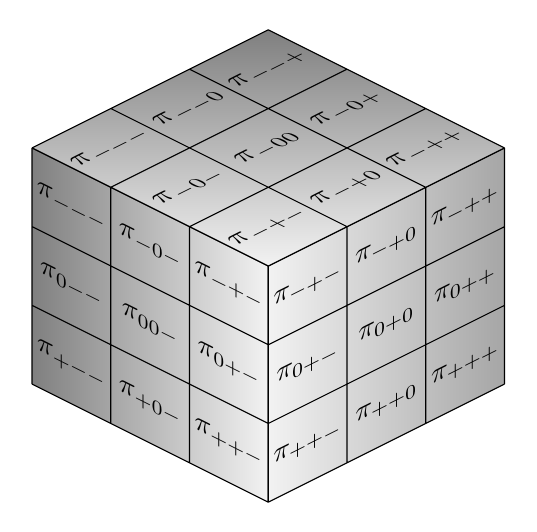
\begin{tikzpicture}[every node/.style={minimum size=1cm},on grid]
\begin{scope}[every node/.append style={yslant=-0.5},yslant=-0.5]
  \shade[right color=gray!10, left color=black!50] (0,0) rectangle +(3,3);
  \node at (0.5,2.5) {$\pi_{---}$};
  \node at (1.5,2.5) {$\pi_{-0-}$};
  \node at (2.5,2.5) {$\pi_{-+-}$};
  \node at (0.5,1.5) {$\pi_{0--}$};
  \node at (1.5,1.5) {$\pi_{00-}$};
  \node at (2.5,1.5) {$\pi_{0+-}$};
  \node at (0.5,0.5) {$\pi_{+--}$};
  \node at (1.5,0.5) {$\pi_{+0-}$};
  \node at (2.5,0.5) {$\pi_{++-}$};
  \draw (0,0) grid (3,3);
\end{scope}
\begin{scope}[every node/.append style={yslant=0.5},yslant=0.5]
  \shade[right color=gray!70,left color=gray!10] (3,-3) rectangle +(3,3);
  \node at (3.5,-0.5) {$\pi_{-+-}$};
  \node at (4.5,-0.5) {$\pi_{-+0}$};
  \node at (5.5,-0.5) {$\pi_{-++}$};
  \node at (3.5,-1.5) {$\pi_{0+-}$};
  \node at (4.5,-1.5) {$\pi_{0+0}$};
  \node at (5.5,-1.5) {$\pi_{0++}$};
  \node at (3.5,-2.5) {$\pi_{++-}$};
  \node at (4.5,-2.5) {$\pi_{++0}$};
  \node at (5.5,-2.5) {$\pi_{+++}$};
  \draw (3,-3) grid (6,0);
\end{scope}
\begin{scope}[every node/.append style={
    yslant=0.5,xslant=-1},yslant=0.5,xslant=-1
  ]
  \shade[bottom color=gray!10, top color=black!50] (6,3) rectangle +(-3,-3);
  \node at (3.5,2.5) {$\pi_{---}$};
  \node at (3.5,1.5) {$\pi_{-0-}$};
  \node at (3.5,0.5) {$\pi_{-+-}$};
  \node at (4.5,2.5) {$\pi_{--0}$};
  \node at (4.5,1.5) {$\pi_{-00}$};
  \node at (4.5,0.5) {$\pi_{-+0}$};
  \node at (5.5,2.5) {$\pi_{--+}$};
  \node at (5.5,1.5) {$\pi_{-0+}$};
  \node at (5.5,0.5) {$\pi_{-++}$};
  \draw (3,0) grid (6,3);
\end{scope}
\end{tikzpicture}


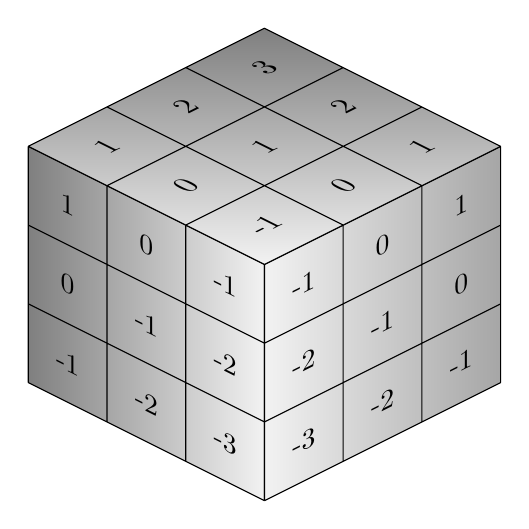
\begin{tikzpicture}[every node/.style={minimum size=1cm},on grid]
\begin{scope}[every node/.append style={yslant=-0.5},yslant=-0.5]
  \shade[right color=gray!10, left color=black!50] (0,0) rectangle +(3,3);
  \node at (0.5,2.5) {1};
  \node at (1.5,2.5) {0};
  \node at (2.5,2.5) {-1};
  \node at (0.5,1.5) {0};
  \node at (1.5,1.5) {-1};
  \node at (2.5,1.5) {-2};
  \node at (0.5,0.5) {-1};
  \node at (1.5,0.5) {-2};
  \node at (2.5,0.5) {-3};
  \draw (0,0) grid (3,3);
\end{scope}
\begin{scope}[every node/.append style={yslant=0.5},yslant=0.5]
  \shade[right color=gray!70,left color=gray!10] (3,-3) rectangle +(3,3);
  \node at (3.5,-0.5) {-1};
  \node at (4.5,-0.5) {0};
  \node at (5.5,-0.5) {1};
  \node at (3.5,-1.5) {-2};
  \node at (4.5,-1.5) {-1};
  \node at (5.5,-1.5) {0};
  \node at (3.5,-2.5) {-3};
  \node at (4.5,-2.5) {-2};
  \node at (5.5,-2.5) {-1};
  \draw (3,-3) grid (6,0);
\end{scope}
\begin{scope}[every node/.append style={
    yslant=0.5,xslant=-1},yslant=0.5,xslant=-1
  ]
  \shade[bottom color=gray!10, top color=black!50] (6,3) rectangle +(-3,-3);
  \node at (3.5,2.5) {1};
  \node at (3.5,1.5) {0};
  \node at (3.5,0.5) {-1};
  \node at (4.5,2.5) {2};
  \node at (4.5,1.5) {1};
  \node at (4.5,0.5) {0};
  \node at (5.5,2.5) {3};
  \node at (5.5,1.5) {2};
  \node at (5.5,0.5) {1};
  \draw (3,0) grid (6,3);
\end{scope}
\end{tikzpicture}


\newpage
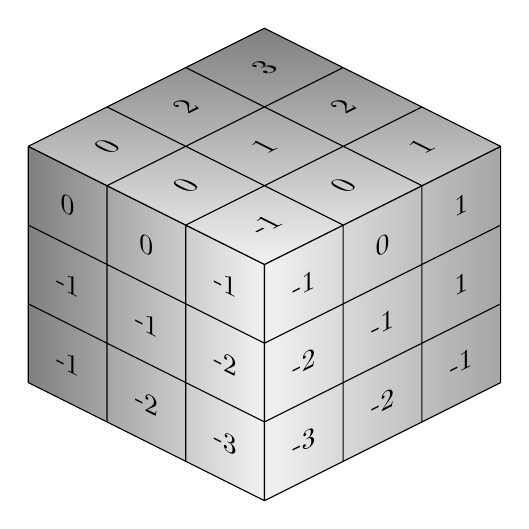
\begin{tikzpicture}[every node/.style={minimum size=1cm},on grid]
\begin{scope}[every node/.append style={yslant=-0.5},yslant=-0.5]
  \shade[right color=gray!10, left color=black!50] (0,0) rectangle +(3,3);
  \node at (0.5,2.5) {0};
  \node at (1.5,2.5) {0};
  \node at (2.5,2.5) {-1};
  \node at (0.5,1.5) {-1};
  \node at (1.5,1.5) {-1};
  \node at (2.5,1.5) {-2};
  \node at (0.5,0.5) {-1};
  \node at (1.5,0.5) {-2};
  \node at (2.5,0.5) {-3};
  \draw (0,0) grid (3,3);
\end{scope}
\begin{scope}[every node/.append style={yslant=0.5},yslant=0.5]
  \shade[right color=gray!70,left color=gray!10] (3,-3) rectangle +(3,3);
  \node at (3.5,-0.5) {-1};
  \node at (4.5,-0.5) {0};
  \node at (5.5,-0.5) {1};
  \node at (3.5,-1.5) {-2};
  \node at (4.5,-1.5) {-1};
  \node at (5.5,-1.5) {1};
  \node at (3.5,-2.5) {-3};
  \node at (4.5,-2.5) {-2};
  \node at (5.5,-2.5) {-1};
  \draw (3,-3) grid (6,0);
\end{scope}
\begin{scope}[every node/.append style={
    yslant=0.5,xslant=-1},yslant=0.5,xslant=-1
  ]
  \shade[bottom color=gray!10, top color=black!50] (6,3) rectangle +(-3,-3);
  \node at (3.5,2.5) {0};
  \node at (3.5,1.5) {0};
  \node at (3.5,0.5) {-1};
  \node at (4.5,2.5) {2};
  \node at (4.5,1.5) {1};
  \node at (4.5,0.5) {0};
  \node at (5.5,2.5) {3};
  \node at (5.5,1.5) {2};
  \node at (5.5,0.5) {1};
  \draw (3,0) grid (6,3);
\end{scope}
\end{tikzpicture}


\newpage

\begin{center}
\begin{tabular}{r | r | r | r | c c c | }
 \multicolumn{3}{r}{} & \multicolumn{1}{r}{} &	\multicolumn{3}{c}{$t$} \\ \cline{5-7}
 \multicolumn{3}{r}{} & 		& \textbf{-} & \textbf{0} & \textbf{+} \\ \cline{2-2} \cline{4-7}
&     &		&    \textbf{-} & $\pi_{---}$	& $\pi_{--0}$	& $\pi_{--+}$ \\ 
&  $-$ &$t-1$ & \textbf{0} & $\pi_{-0-}$	& $\pi_{-00}$	& $\pi_{-0+}$	\\
     &   &		&    \textbf{+} & $\pi_{-+-}$	& $\pi_{-+0}$	& $\pi_{-++}$ \\ \cline{2-2} \cline{4-7}
     &   &		&    \textbf{-} & $\pi_{0--}$	& $\pi_{0-0}$	& $\pi_{0-+}$ \\ 
$t-2$ & $0$   &$t-1$ & \textbf{0} & $\pi_{00-}$	& $\pi_{000}$	& $\pi_{00+}$	\\
     &   &		&    \textbf{+} & $\pi_{0+-}$	& $\pi_{0+0}$	& $\pi_{0++}$ \\ \cline{2-2} \cline{4-7}
     &   &		&    \textbf{-} & $\pi_{+--}$	& $\pi_{+-0}$	& $\pi_{+-+}$ \\ 
&$+$   &$t-1$ & \textbf{0} & $\pi_{+0-}$	& $\pi_{+00}$	& $\pi_{+0+}$	\\
     &   &		&    \textbf{+} & $\pi_{++-}$	& $\pi_{++0}$	& $\pi_{+++}$ \\ \cline{2-2} \cline{4-7}
		
\end{tabular}    
\end{center}

\begin{center}
\begin{tabular}{r | r | r | r | c c c | }
 \multicolumn{3}{r}{} & \multicolumn{1}{r}{} &	\multicolumn{3}{c}{$t$} \\ \cline{5-7}
 \multicolumn{3}{r}{} & 		& \textbf{-} & \textbf{0} & \textbf{+} \\ \cline{2-2} \cline{4-7}
&     &		&    \textbf{-} & $1$	& $2$	& $3$ \\ 
&  $-$ &$t-1$ & \textbf{0} & $0$	& $1$	& $2$	\\
     &   &		&    \textbf{+} & $-1$	& $0$	& $1$ \\ \cline{2-2} \cline{4-7}

     &   &		&    \textbf{-} & $0$	& $1$	& $2$ \\ 
$t-2$ & $0$   &$t-1$ & \textbf{0} & $-1$	& $0$	& $1$	\\
     &   &		&    \textbf{+} & $-2$	& $-1$	& $0$ \\ \cline{2-2} \cline{4-7}

     &   &		&    \textbf{-} & $-1$	& $0$	& $1$ \\ 
&$+$   &$t-1$ & \textbf{0} & $-2$	& $-1$	& $0$	\\
     &   &		&    \textbf{+} & $-3$	& $-2$	& $-1$ \\ \cline{2-2} \cline{4-7}
		
\end{tabular}    
\end{center}


\newpage

\begin{center}
\begin{tabular}{r | r | r | r | r | r | c c c | }
 \multicolumn{5}{r}{} & \multicolumn{1}{r}{} &	\multicolumn{3}{c}{$t$} \\ \cline{7-9}
 \multicolumn{5}{r}{} & 		& \textbf{-} & \textbf{0} & \textbf{+} \\ \cline{2-2} \cline{4-4} \cline{6-9}
& & &	& &   \textbf{-} & $\pi_{----}$	& $\pi_{---0}$	& $\pi_{---+}$ \\ 
& & &  $-$ &$t-1$ & \textbf{0} & $\pi_{--0-}$	& $\pi_{--00}$	& $\pi_{--0+}$	\\
& &      &   &		&    \textbf{+} & $\pi_{--+-}$	& $\pi_{--+0}$	& $\pi_{--++}$ \\ \cline{4-4} \cline{6-9}
& &      &   &		&    \textbf{-} & $\pi_{-0--}$	& $\pi_{-0-0}$	& $\pi_{-0-+}$ \\ 
& $-$ & $t-2$ & $0$   &$t-1$ & \textbf{0} & $\pi_{-00-}$	& $\pi_{-000}$	& $\pi_{-00+}$	\\
& &      &   &		&    \textbf{+} & $\pi_{-0+-}$	& $\pi_{-0+0}$	& $\pi_{-0++}$ \\  \cline{4-4} \cline{6-9}
& &      &   &		&    \textbf{-} & $\pi_{-+--}$	& $\pi_{-+-0}$	& $\pi_{-+-+}$ \\ 
& & &$+$   &$t-1$ & \textbf{0} & $\pi_{-+0-}$	& $\pi_{-+00}$	& $\pi_{-+0+}$	\\
& &      &   &		&    \textbf{+} & $\pi_{-++-}$	& $\pi_{-++0}$	& $\pi_{-+++}$ \\ \cline{2-2} \cline{4-4} \cline{6-9}

& &     &	&	&    \textbf{-} & $\pi_{0---}$	& $\pi_{0--0}$	& $\pi_{0--+}$ \\ 
& & &  $-$ &$t-1$ & \textbf{0} & $\pi_{0-0-}$	& $\pi_{0-00}$	& $\pi_{0-0+}$	\\
& &      &   &		&    \textbf{+} & $\pi_{0-+-}$	& $\pi_{0-+0}$	& $\pi_{0-++}$ \\ \cline{4-4} \cline{6-9}
& &      &   &		&    \textbf{-} & $\pi_{00--}$	& $\pi_{00-0}$	& $\pi_{00-+}$ \\ 
$t-3$ & $0$ & $t-2$ & $0$   &$t-1$ & \textbf{0} & $\pi_{000-}$	& $\pi_{0000}$	& $\pi_{000+}$	\\
& &      &   &		&    \textbf{+} & $\pi_{00+-}$	& $\pi_{00+0}$	& $\pi_{00++}$ \\ \cline{4-4} \cline{6-9}
& &      &   &		&    \textbf{-} & $\pi_{++--}$	& $\pi_{++-0}$	& $\pi_{++-+}$ \\ 
& & &$+$   &$t-1$ & \textbf{0} & $\pi_{++0-}$	& $\pi_{++00}$	& $\pi_{++0+}$	\\
& &      &   &		&    \textbf{+} & $\pi_{+++-}$	& $\pi_{+++0}$	& $\pi_{++++}$ \\ \cline{2-2} \cline{4-4} \cline{6-9}

& &     &	&	&    \textbf{-} & $\pi_{+---}$	& $\pi_{+--0}$	& $\pi_{+--+}$ \\ 
& & &  $-$ &$t-1$ & \textbf{0} & $\pi_{+-0-}$	& $\pi_{+-00}$	& $\pi_{+-0+}$	\\
& &      &   &		&    \textbf{+} & $\pi_{+-+-}$	& $\pi_{+-+0}$	& $\pi_{+-++}$ \\ \cline{4-4} \cline{6-9}
& &      &   &		&    \textbf{-} & $\pi_{+0--}$	& $\pi_{+0-0}$	& $\pi_{+0-+}$ \\ 
& $+$  & $t-2$ & $0$   &$t-1$ & \textbf{0} & $\pi_{+00-}$	& $\pi_{+000}$	& $\pi_{+00+}$	\\
& &      &   &		&    \textbf{+} & $\pi_{+0+-}$	& $\pi_{+0+0}$	& $\pi_{+0++}$ \\ \cline{4-4} \cline{6-9}
& &      &   &		&    \textbf{-} & $\pi_{++--}$	& $\pi_{++-0}$	& $\pi_{++-+}$ \\ 
& & &$+$   &$t-1$ & \textbf{0} & $\pi_{++0-}$	& $\pi_{++00}$	& $\pi_{++0+}$	\\
& &      &   &		&    \textbf{+} & $\pi_{+++-}$	& $\pi_{+++0}$	& $\pi_{++++}$ \\ \cline{2-2} \cline{4-4} \cline{6-9}
\end{tabular}    
\end{center}


\begin{center}
\begin{tabular}{r | r | r | r | r | r | c c c | }
 \multicolumn{5}{r}{} & \multicolumn{1}{r}{} &	\multicolumn{3}{c}{$t$} \\ \cline{7-9}
 \multicolumn{5}{r}{} & 		& \textbf{-} & \textbf{0} & \textbf{+} \\ \cline{2-2} \cline{4-4} \cline{6-9}

& & &	& &   \textbf{-} & $2$	& $3$	& $4$ \\ 
& & &  $-$ &$t-1$ & \textbf{0} & $1$	& $2$	& $3$	\\
& &      &   &		&    \textbf{+} & $0$	& $1$	& $2$ \\ \cline{4-4} \cline{6-9}

& &      &   &		&    \textbf{-} & $-1$	& $0$	& $1$ \\ 
& $-$ & $t-2$ & $0$   &$t-1$ & \textbf{0} & $0$	& $1$	& $2$	\\
& &      &   &		&    \textbf{+} & $-1$	& $0$	& $1$ \\  \cline{4-4} \cline{6-9}

& &      &   &		&    \textbf{-} & $0$	& $1$	& $2$ \\ 
& & &$+$   &$t-1$ & \textbf{0} & $-1$	& $0$	& $1$	\\
& &      &   &		&    \textbf{+} & $-2$	& $-1$	& $0$ \\ \cline{2-2} \cline{4-4} \cline{6-9}

& &     &	&	&    \textbf{-} & $1$	& $2$	& $3$ \\ 
& & &  $-$ &$t-1$ & \textbf{0} & $0$	& $1$	& $2$	\\
& &      &   &		&    \textbf{+} & $-1$	& $0$	& $1$ \\ \cline{4-4} \cline{6-9}

& &      &   &		&    \textbf{-} & $0$	& $1$	& $2$ \\ 
$t-3$ & $0$ & $t-2$ & $0$   &$t-1$ & \textbf{0} & $-1$	& $0$	& $1$	\\
& &      &   &		&    \textbf{+} & $-2$	& $-1$	& $0$ \\ \cline{4-4} \cline{6-9}

& &      &   &		&    \textbf{-} & $-1$	& $0$	& $1$ \\ 
& & &$+$   &$t-1$ & \textbf{0} & $-2$	& $-1$	& $0$	\\
& &      &   &		&    \textbf{+} & $-3$	& $-2$	& $-1$ \\ \cline{2-2} \cline{4-4} \cline{6-9}

& &     &	&	&    \textbf{-} & $0$	& $1$	& $2$ \\ 
& & &  $-$ &$t-1$ & \textbf{0} & $-1$	& $0$	& $1$	\\
& &      &   &		&    \textbf{+} & $-2$	& $-1$	& $0$ \\ \cline{4-4} \cline{6-9}

& &      &   &		&    \textbf{-} & $-1$	& $0$	& $1$ \\ 
& $+$  & $t-2$ & $0$   &$t-1$ & \textbf{0} & $-2$	& $-1$	& $0$	\\
& &      &   &		&    \textbf{+} & $-3$	& $-2$	& $-1$ \\ \cline{4-4} \cline{6-9}

& &      &   &		&    \textbf{-} & $-2$	& $-1$	& $0$ \\ 
& & &$+$   &$t-1$ & \textbf{0} & $-3$	& $-2$	& $-1$	\\
& &      &   &		&    \textbf{+} & $-4$	& $-3$	& $-2$ \\ \cline{2-2} \cline{4-4} \cline{6-9}
\end{tabular}    
\end{center}




\newpage

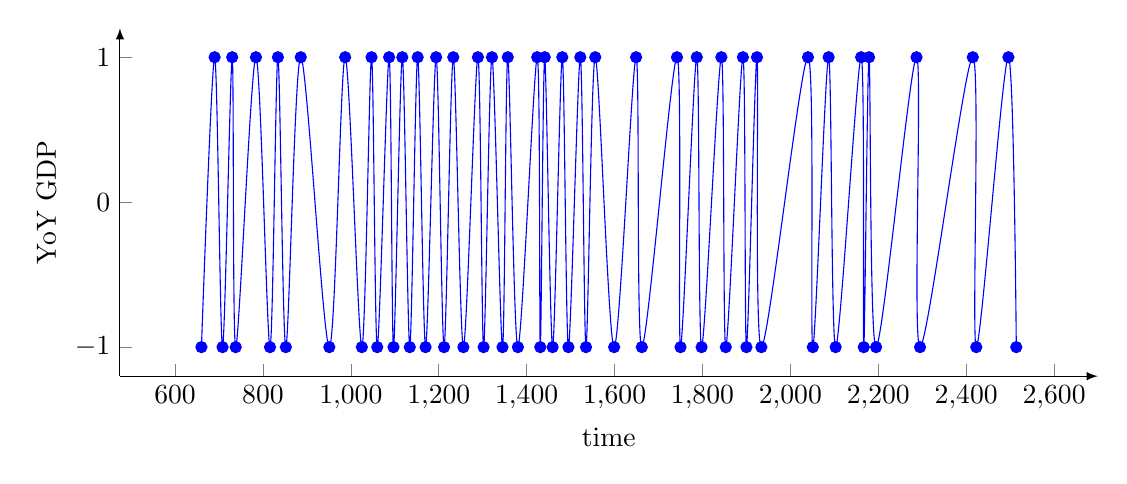
\begin{tikzpicture}
\begin{axis}[
    domain=0:6*pi,
    samples=100,
    axis lines*=left, 
    axis line style={->},
%    xtick={1.6, 4.8, 7.9, 11, 14.1, 17.3}, ytick=\empty,
    width=14cm, height=6cm,
    xlabel={time}, 
    ylabel={YoY GDP}
]       
    \addplot[smooth,mark=*,blue] plot coordinates {        (660,-1)
        (690,1)
        (708,-1)
        (730,1) (738,-1)
    (784,1)	(816,-1)
    (834,1)	(852,-1)
    (886,1)	(951,-1)
    (987,1)	(1025,-1)
    (1047,1)	(1060,-1)
    (1087,1)	(1097,-1)
    (1117,1)	(1134,-1)
    (1152,1)	(1170,-1)
    (1194,1)	(1212,-1)
    (1233,1)	(1256,-1)
    (1289,1)	(1302,-1)
    (1321,1)	(1345,-1)
    (1357,1)	(1380,-1)
    (1424,1)	(1431,-1)
    (1441,1)	(1459,-1)
    (1481,1)	(1495,-1)
    (1522,1)	(1535,-1)
    (1556,1)	(1599,-1)
    (1649,1)	(1662,-1)
    (1742,1)	(1750,-1)
    (1787,1)	(1798,-1)
    (1843,1)	(1853,-1)
    (1892,1)	(1900,-1)
    (1924,1)	(1934,-1)
    (2040,1)	(2051,-1)
    (2087,1)	(2103,-1)
    (2161,1)	(2167,-1)
    (2179,1)	(2195,-1)
    (2287,1)	(2295,-1)
    (2415,1)	(2423,-1)
    (2496,1)	(2514,-1)
    };
\end{axis}
\end{tikzpicture}


\newpage


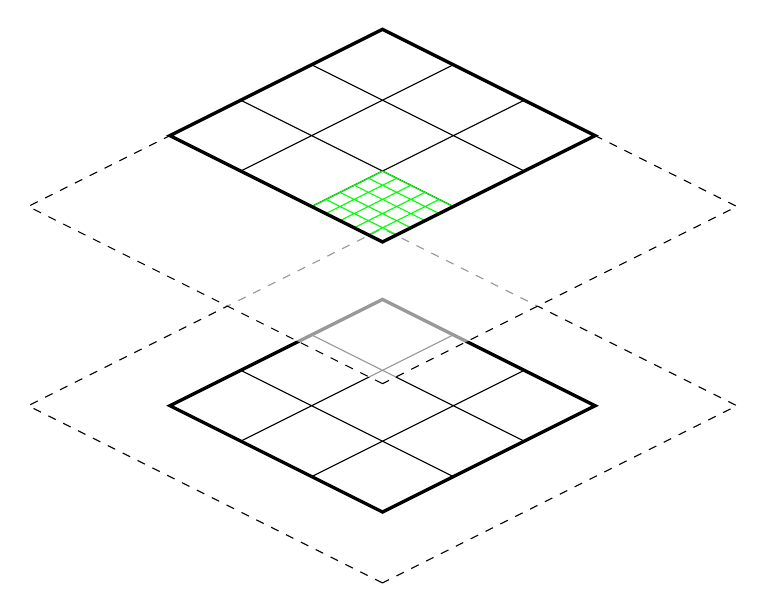
\begin{tikzpicture}[scale=.9,every node/.style={minimum size=1cm},on grid]
		
    %slanting: production of a set of n 'laminae' to be piled up. N=number of grids.
    	
    \begin{scope}[
    	yshift=90,every node/.append style={
    	yslant=0.5,xslant=-1},yslant=0.5,xslant=-1
    	             ]
    	\fill[white,fill opacity=.9] (0,0) rectangle (5,5);
    	\draw[step=10mm, black] (1,1) grid (4,4);
    	\draw[black,very thick] (1,1) rectangle (4,4);
    	\draw[black,dashed] (0,0) rectangle (5,5);
    \end{scope}
    	
    \begin{scope}[
    	yshift=170,every node/.append style={
    	    yslant=0.5,xslant=-1},yslant=0.5,xslant=-1
    	  ]
        \fill[white,fill opacity=0.6] (0,0) rectangle (5,5);
        \draw[step=10mm, black] (2,2) grid (5,5);
        \draw[step=2mm, green] (2,2) grid (3,3);
        \draw[black,very thick] (2,2) rectangle (5,5);
        \draw[black,dashed] (0,0) rectangle (5,5);
    \end{scope}
    	
\end{tikzpicture}




\newpage
\subsubsection{t-3 vs t-2 vs t-1 vs t}

\begin{center}
\begin{tabular}{r | r | r | r | r | r | c c c | }
 \multicolumn{5}{r}{} & \multicolumn{1}{r}{} &	\multicolumn{3}{c}{$t$} \\ \cline{7-9}
 \multicolumn{5}{r}{} & 		& \textbf{-} & \textbf{0} & \textbf{+} \\ \cline{2-2} \cline{4-4} \cline{6-9}
&&&&&   \textbf{-} & $\pi_{----}$	& $\pi_{---0}$	& $\pi_{---+}$ \\ 
&&&  $-$ &$t-1$ & \textbf{0} & $\pi_{--0-}$	& $\pi_{--00}$	& $\pi_{--0+}$	\\
&&&&&    \textbf{+} & $\pi_{--+-}$	& $\pi_{--+0}$	& $\pi_{--++}$ \\ \cline{4-4} \cline{6-9}
&&&&&    \textbf{-} & $\pi_{-0--}$	& $\pi_{-0-0}$	& $\pi_{-0-+}$ \\ 
& $-$ & $t-2$ & $0$   &$t-1$ & \textbf{0} & $\pi_{-00-}$	& $\pi_{-000}$	& $\pi_{-00+}$	\\
&&&&&    \textbf{+} & $\pi_{-0+-}$	& $\pi_{-0+0}$	& $\pi_{-0++}$ \\  \cline{4-4} \cline{6-9}
&&&&&    \textbf{-} & $\pi_{-+--}$	& $\pi_{-+-0}$	& $\pi_{-+-+}$ \\ 
&&&$+$   &$t-1$ & \textbf{0} & $\pi_{-+0-}$	& $\pi_{-+00}$	& $\pi_{-+0+}$	\\
&&&&&    \textbf{+} & $\pi_{-++-}$	& $\pi_{-++0}$	& $\pi_{-+++}$ \\ \cline{2-2} \cline{4-4} \cline{6-9}

&&&&&    \textbf{-} & $\pi_{0---}$	& $\pi_{0--0}$	& $\pi_{0--+}$ \\ 
&&& $-$ &$t-1$ & \textbf{0} & $\pi_{0-0-}$	& $\pi_{0-00}$	& $\pi_{0-0+}$	\\
&&&&& \textbf{+} & $\pi_{0-+-}$	& $\pi_{0-+0}$	& $\pi_{0-++}$ \\ \cline{4-4} \cline{6-9}
&&&&&    \textbf{-} & $\pi_{00--}$	& $\pi_{00-0}$	& $\pi_{00-+}$ \\ 
$t-3$ & $0$ & $t-2$ & $0$   &$t-1$ & \textbf{0} & $\pi_{000-}$	& $\pi_{0000}$	& $\pi_{000+}$	\\
&&&&&    \textbf{+} & $\pi_{00+-}$	& $\pi_{00+0}$	& $\pi_{00++}$ \\ \cline{4-4} \cline{6-9}
&&&&& \textbf{-} & $\pi_{++--}$	& $\pi_{++-0}$	& $\pi_{++-+}$ \\ 
& & &$+$   &$t-1$ & \textbf{0} & $\pi_{++0-}$	& $\pi_{++00}$	& $\pi_{++0+}$	\\
&&&&& \textbf{+} & $\pi_{+++-}$	& $\pi_{+++0}$	& $\pi_{++++}$ \\ \cline{2-2} \cline{4-4} \cline{6-9}

&&&&& \textbf{-} & $\pi_{+---}$	& $\pi_{+--0}$	& $\pi_{+--+}$ \\ 
&&& $-$ &$t-1$ & \textbf{0} & $\pi_{+-0-}$	& $\pi_{+-00}$	& $\pi_{+-0+}$	\\
&&&&& \textbf{+} & $\pi_{+-+-}$	& $\pi_{+-+0}$	& $\pi_{+-++}$ \\ \cline{4-4} \cline{6-9}
&&&&& \textbf{-} & $\pi_{+0--}$	& $\pi_{+0-0}$	& $\pi_{+0-+}$ \\ 
& $+$  & $t-2$ & $0$   &$t-1$ & \textbf{0} & $\pi_{+00-}$	& $\pi_{+000}$	& $\pi_{+00+}$	\\
&&&&& \textbf{+} & $\pi_{+0+-}$ & $\pi_{+0+0}$	& $\pi_{+0++}$ \\ \cline{4-4} \cline{6-9}
&&&&& \textbf{-} & $\pi_{++--}$ & $\pi_{++-0}$	& $\pi_{++-+}$ \\ 
&&&$+$   &$t-1$ & \textbf{0} & $\pi_{++0-}$	& $\pi_{++00}$	& $\pi_{++0+}$	\\
&&&&& \textbf{+} & $\pi_{+++-}$	& $\pi_{+++0}$	& $\pi_{++++}$ \\ \cline{2-2} \cline{4-4} \cline{6-9}
\end{tabular}    
\end{center}




\begin{center}
\begin{tabular}{r | r | r | r | r | r | c c c | }
 \multicolumn{5}{r}{} & \multicolumn{1}{r}{} &	\multicolumn{3}{c}{$t$} \\ \cline{7-9}
 \multicolumn{5}{r}{} & 		& \textbf{-} & \textbf{0} & \textbf{+} \\ \cline{2-2} \cline{4-4} \cline{6-9}

&&&&& \textbf{-}            & $0$	& $3$	& $4$ \\ 
&&&$-$&$t-1$& \textbf{0}    & $1$	& $2$	& $3$	\\
&&&&&\textbf{+}             & $0$	& $1$	& $2$ \\ \cline{4-4} \cline{6-9}

&&&&&\textbf{-}             & $0$	& $0$	& $1$ \\ 
&$-$&$t-2$&$0$&$t-1$&\textbf{0} & $0$	& $1$	& $2$	\\
&&&&&\textbf{+}                 & $-1$	& $0$	& $1$ \\  \cline{4-4} \cline{6-9}

&&&&&\textbf{-}                 & $0$	& $1$	& $2$ \\ 
&&&$+$   &$t-1$ & \textbf{0}    & $-1$	& $0$	& $1$	\\
&&&&&\textbf{+}                 & $-2$	& $-1$	& $0$ \\ \cline{2-2} \cline{4-4} \cline{6-9}

&&&&& \textbf{-}                    & $1$	& $2$	& $3$ \\ 
&&&$-$&$t-1$&\textbf{0}             & $0$	& $0$	& $2$	\\
&&&&&\textbf{+}                     & $-1$	& $0$	& $1$ \\ \cline{4-4} \cline{6-9}

&&&&&\textbf{-}                     & $0$	& $1$	& $2$ \\ 
$t-3$&$0$&$t-2$&$0$&$t-1$&\textbf{0}& $-1$	& $0$	& $1$	\\
&&&&&\textbf{+}                     & $-2$	& $-1$	& $0$ \\ \cline{4-4} \cline{6-9}

&&&&&\textbf{-}                     & $-1$	& $0$	& $1$ \\ 
&&&$+$   &$t-1$ & \textbf{0}        & $-2$	& $0$	& $0$	\\
&&&&&\textbf{+}                     & $-3$	& $-2$	& $-1$ \\ \cline{2-2} \cline{4-4} \cline{6-9}

& &     &	&	&    \textbf{-}     & $0$	& $1$	& $2$ \\ 
&&&  $-$ &$t-1$ & \textbf{0}        & $-1$	& $0$	& $1$	\\
&&&&&\textbf{+}                     & $-2$	& $-1$	& $0$ \\ \cline{4-4} \cline{6-9}

&&&&&\textbf{-}                     & $-1$	& $0$	& $1$ \\ 
&$+$&$t-2$&$0$&$t-1$&\textbf{0}     & $-2$	& $-1$	& $0$	\\
&&&&&\textbf{+}                     & $-3$	& $-2$	& $0$ \\ \cline{4-4} \cline{6-9}

&&&&&\textbf{-}                     & $-2$	& $-1$	& $0$ \\ 
&&&$+$   &$t-1$ & \textbf{0}        & $-3$	& $-2$	& $-1$	\\
&&&&&\textbf{+}                     & $-4$	& $-3$	& $0$ \\ \cline{2-2} \cline{4-4} \cline{6-9}
\end{tabular}    
\end{center}



\begin{figure}[H]
     \centering
    \begin{tikzpicture}  \footnotesize
   \draw [thin, black, ->] (0,0) -- (0, 2.2)      % draw y-axis line

    \draw [thin, black, ->] (0,0) -- (2.2 ,0)      % draw x-axis line

    \draw [draw=black,ultra thick] (0.5,1) -- (1.5,1);% draw the graph

    \node [left] at (0,0.5) {negative};                
    \node [left] at (0,1) {neutral};                
    \node [left] at (0,1.5) {positive};                
    \node [below] at (0.5,0) {$t-1$};            
    \node [below] at (1.5,0) {$t$};               
    \end{tikzpicture}
      \caption{wazazaza}
    \label{fig:explanation of Var and BSI}
\end{figure}


\end{document}